\documentclass[12pt]{article}
\usepackage{graphicx}
\usepackage{algpseudocode}
\usepackage{algorithm}
\usepackage{booktabs}
\usepackage[style=alphabetic, backend=biber]{biblatex}
\usepackage{setspace}

\graphicspath{ {./images/} }

\addbibresource{references.bib}

% Preamble
\setlength{\parindent}{0pt}
\linespread{2}

% Document Information
\title{
    Computer Science \\
    \vspace{1cm}
    Ray Tracing Voxels with Hardware Acceleration in Real-Time \\
    \vspace{1cm}
    \large Is hardware accelerated voxel ray tracing feasible on consumer hardware for real-time applications? \\
    \vspace{1cm}
    \large Word Count: 3975
    }
\author{}
\date{2024}

% Begin Document
\begin{document}

% Title Page
\maketitle
\clearpage

% Table of Contents
\tableofcontents
\clearpage


\clearpage

\section{Introduction}

This essay is about the performance analysis of hardware accelerated voxel ray tracing.
When researching about this topic, there was no performance analysis of hardware accelerated voxel ray tracing beforehand.

In this essay, general overview of ray tracing and the process on hardware is explained,
which is greatly simplified and does not cover all the details. Finally, the methodology of
ray tracing voxels and the results of the performance analysis are presented.

\subsection{Ray Tracing}

The following has been discussed in \parencite{NVIDIA:Raytracing} and \parencite{NVIDIA:RTGems2}.
Ray tracing is a method used to calculate where a given ray (line), intersects
with the objects in an environment. It is used to simulate light rays because light rays
travel in straight lines and interact with objects in the environment.
Finding the intersection is essential to simulate the light bouncing off the objects and this essay
focuses on the performance of this process.
This process is utilized in film production, video games, engineering,
architectural visualization, and many other fields that simulate light.
The term ray tracing is used interchangeably with path tracing.
Path tracing is the process of simulating light paths in the environment where it utilizes ray tracing to find intersections.

\begin{figure}[H]
    \begin{center}
        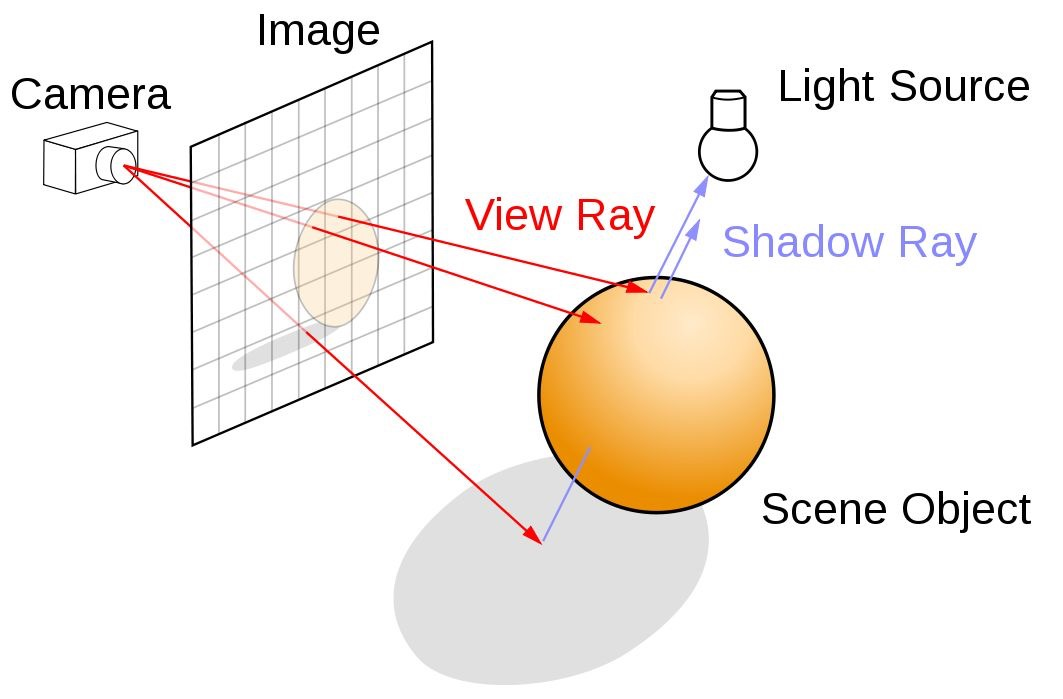
\includegraphics[scale=0.22]{RayTracingImage}
    \end{center}
    \caption{Simplified visualization of the ray tracing process. Note that the rays originate from the camera whereas in reality the rays originate from the light source.}
    \label{fig:RayTracingImage}
\end{figure}

Ray tracing is a highly parallelizable process perfectly suited for GPUs because each ray can be calculated independently of each other.
However, due to how computationally expensive the
process is, it is not feasible to do in real-time without dedicated hardware
acceleration. Due to those limitations, it was only used in non-real-time
applications such as film production. Hardware acceleration ray tracing was introduced in 2018 by NVIDIA \parencite{NVIDIA:DXR-Intro}.
This has allowed real-time applications to leverage ray-tracing such as rendering applications, video games, and visualizations.

\subsection{Voxels}

Voxels are a medium to represent 3 dimensional (3D) data. It is similar to pixels in 2 dimensional images,
but in 3D space. Essentially, voxels are cubes that are located in 3D space.
They are used in visualization applications, and video games.
Voxels are a convenient data representation format, because they represent
volumetric data, which is difficult to represent with traditional with polygons that the GPU is designed to handle.
Environment scans and medical imaging data are examples of volumetric data.
For example, LiDAR sensors are used to scan an environment which output a collection of points in 3D space.
These points can be converted to voxels efficiently, because each point in 3D space can be represented as a voxel \parencite{NOS:LiDAR}.

\begin{figure}[H]
    \begin{center}
        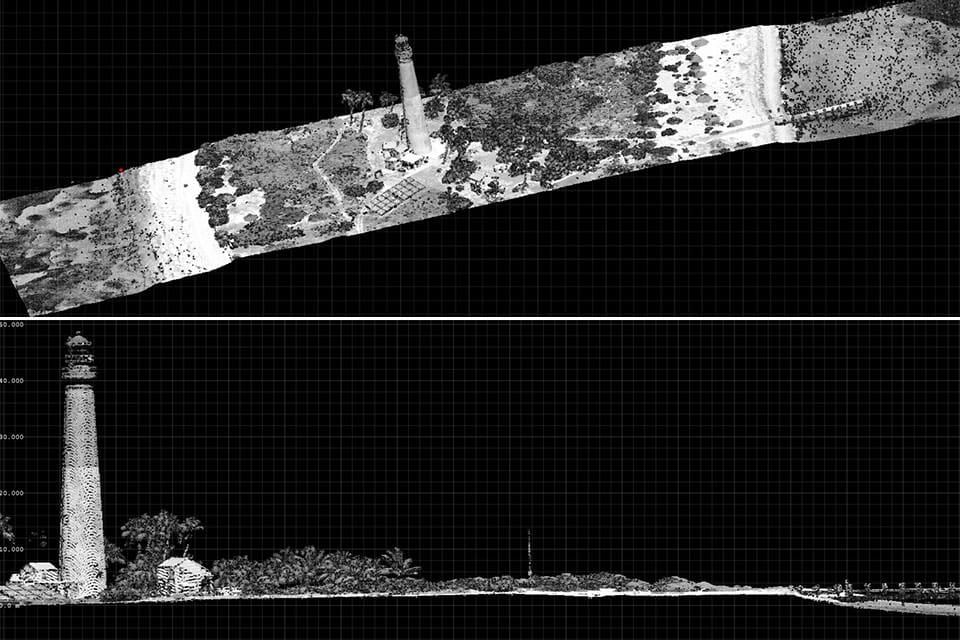
\includegraphics[scale=0.4]{LiDAR}
    \end{center}
    \caption{LiDAR scan of an environment represented as voxels in 3D space. \parencite{NOS:LiDAR}}
    \label{fig:LiDAR}
\end{figure}

It is utilized in simulations or visualizations, such as Figure \ref{fig:LiDAR}.
Each voxel can contain data, such as color, or any relevant information,
which can be utilized in simulations or visualizations. With the recent advancements in hardware acceleration
ray tracing, voxel ray tracing has become hardware accelerated. \parencite[Chapter~37]{NVIDIA:RTGems2}

\subsection{Research Question}

Voxels are a convenient data representation format, and ray tracing is a powerful tool to simulate light rays,
it will be interesting to see if it can be viable for use in real-time applications.
Hence, the research question is: {\bf Is hardware accelerated voxel ray tracing feasible on consumer hardware for real-time applications? }
Real-time applications considered are video games, and visualizations that utilize volumetric data in the form of voxels.

Writing an application to analyze this research, requires a deep understanding of the hardware, memory, graphics application programming interfaces (GAPI), graphics programming languages, debugging, etc.
GAPIs allow communication between the application and the GPU.
The GAPIs are designed for industry professionals with years of experience working with GPUs, hence are complex.
Furthermore, debugging is non-trivial, because the algorithms are executed on the GPU, which cannot be debugged with traditional debugging tools.
Understanding all of these topics comfortably may require years of experience. Writing 3000+ lines of code was required to conduct this research, without accounting for rewrites of algorithms, debugging, and testing.

These are the factors that will be considered when evaluating the feasibility:
\begin{itemize}
    \itemsep0em
    \item Can it handle a reasonable number of voxels? (3-15 Million) in real-time?
    \item Does it exceed the memory budget? (1 GB)
\end{itemize}

The range of voxels considered are 3-15 million, because it represents a reasonable amount of data that can be visually shown on a screen.
The performance target is 60+ frames per second (FPS), or below 16.67 milliseconds per frame for the scenes, which is considered
smooth and interactive for real-time applications.

Most consumer GPUs have at least 4 GB of memory, hence a memory budget of 1 GB is reasonable while still leaving memory for other tasks than rendering.
For example, Artificial Intelligence (AI) tasks are common that requires abundant memory.


Following sections will describe the ray tracing process, and the methodology used to evaluate the research question.
After the methodology, the results of the performance analysis will be presented.

\section{Background Information}

\subsection{Path Tracing Algorithm}

To render an image using ray tracing, the path tracing algorithm is used, which can be extremely complicated depending on to what extent the light is simulated.
This essay will use a simple path tracing algorithm, because the focus of the essay is on the performance of the hardware acceleration and not the shading.
A recursive algorithm is used that calculates the color of a pixel by tracing rays into the scene from a virtual camera.
This algorithm leverages ray tracing to simulate light rays in the scene.

\begin{algorithm}[H]
    \caption{Path Tracing Algorithm}
    \label{alg:TraceRay}
    \small
    \setstretch{1.2}
    \begin{algorithmic}[1]
        \State $Emissive \gets 0$
        \Procedure{TraceRay}{$direction, depth$}

        \If{$depth = 0$}
        \State \Return $0$ \Comment {Hit no light source after maximum depth}
        \EndIf

        \State $closestHit \gets \infty$
        \State $hitObject \gets null$

        \For{$object$ in $scene$}
        \State $hit \gets object.Intersect(direction)$
        \If{$hit < closestHit$}
        \State $closestHit \gets hit$
        \State $hitObject \gets object$
        \EndIf
        \EndFor

        \If{$closestHit = \infty$}
        \State $Emissive \gets 1$ \Comment {Sky is a light source}
        \State \Return $background$
        \EndIf
        \State $Emissive \gets hitObject.emissive$
        \If {$hitObject.emissive$} \Comment {If the object is a light source}
        \State \Return $hitObject.Color$
        \EndIf

        \State $newDirection \gets randomDirectionFromObject(hitObject)$ \Comment {Light can come from any direction to the surface}

        \State \Return $object.Color * TraceRay(newDirection, depth - 1)$

        \EndProcedure

        \For{$pixel$ in $image$}
        \State $direction \gets getDirectionForPixel(pixel)$
        \State $color \gets TraceRay(direction, maxDepth) * Emissive$
        \State $image[pixel] \gets color$
        \State $Emissive \gets 0$ \Comment{Reset Emissive}
        \EndFor
    \end{algorithmic}
\end{algorithm}

The pseudocode in Algorithm \ref{alg:TraceRay} shows a simple recursive algorithm for path tracing.
When $TraceRay$ is called, it finds the closest hit in the scene using ray tracing.
It also ensures that the ray does not bounce infinitely by checking the depth.
The $object.Intersect(direction)$ method is the intersection function that returns the intersection point if the ray hits the object.
If the hit object is emissive (light source), then the path is illuminated by the light source, hence the color is returned.
Note that if the path doesn't hit a light source, the path color is multiplied by 0, resulting in a black color. More paths are traced into random directions from the hit object to find possible paths that hit a light source. Multiplication by the object's color and the next ray's color are essential for physically accurate rendering. For example, if a red sphere and a green sphere are close to each other, the red sphere will reflect red light onto the green sphere, which will make the green sphere have hints of red color and vice versa.
Figure \ref{fig:RayTracingImage} shows a visualization of the path tracing algorithm.
Although not in the pseudocode, this recursive algorithm is repeated many times for each pixel each frame, resulting in a realistic image.
The algorithm is approximately the algorithm used in this essay, however the actual implementation is more complex and implemented in a graphics programming language (HLSL), which has 500+ lines of code.

In practice, this algorithm is split into multiple stages for the hardware acceleration pipeline.
The intersection function is the most critical function for achieving real-time ray tracing.
For-loop from line 8 to 14 in Algorithm \ref{alg:TraceRay} is hardware accelerated in GPUs, because it computes the intersection, although the exact implementation is not disclosed by GPU vendors and is more complex and efficient than the pseudocode. \parencite[Part~5]{NVIDIA:RTGems2}
This will be discussed in the next section.

\subsection{Process of Ray Tracing on Hardware}
In this section, the ray tracing process on hardware is explained.

\subsubsection{Acceleration Structures}

Without any optimization algorithms, intersection tests have to be performed for every primitive in the scene to determine the closest hit for a ray.
Primitives are the smallest building blocks of the scene. The GPU only accepts triangles and axis aligned bounding boxes (AABB) as primitives.
AABBs are cuboids of any size, hence perfect for representing voxels.
This essay will use AABB interchangeably with voxels, because voxels are represented as AABBs in the GPU.

Performing an intersection test for every primitive is impractical for scenes with millions of primitives, because each intersection tests require a significant amount of computation.
Doing this for millions of primitives, for millions of pixels, for every frame is not practical.

To mitigate this problem, Acceleration structures (AS) are used to reduce the number of times the intersection tests are performed.
These structures are usually bounding volume hierarchies (BVH) that subdivide the scene into smaller parts until the smallest primitives are reached \parencite{NVIDIA:Raytracing}.

\begin{figure}[H]
    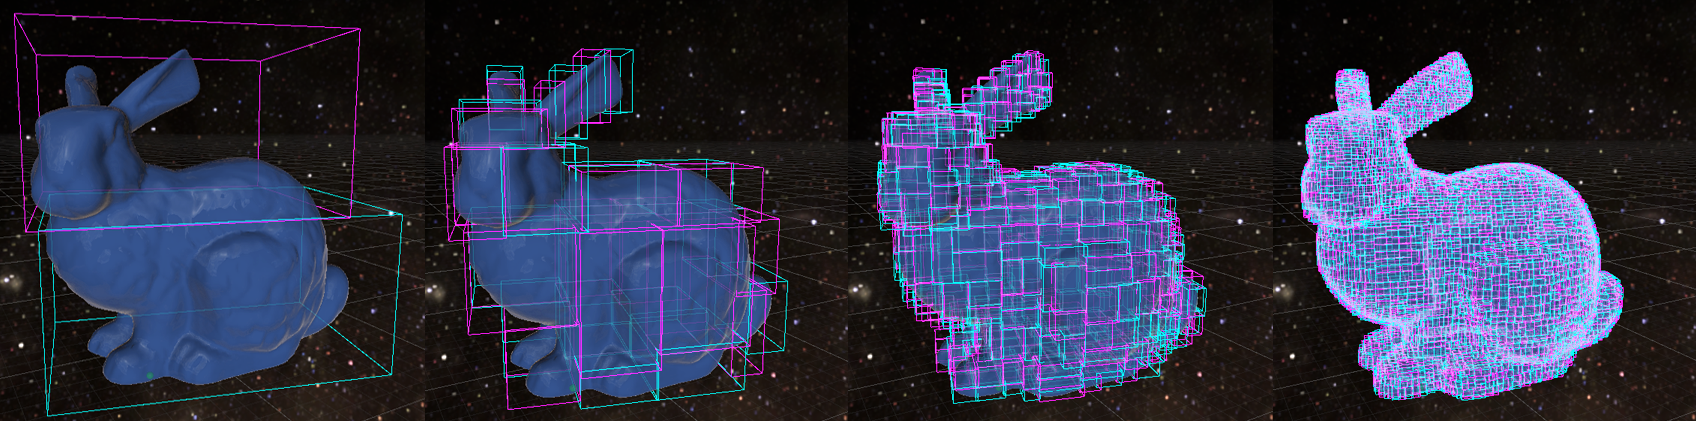
\includegraphics[scale=0.22]{BVH-Visualization}
    \caption{
        Bounding Volume Hierarchy of a bunny.
        The bunny is divided into smaller bounding volumes until the individual triangles are reached.
        \parencite{Medium:BVH-Visualization}
    }
    \label{fig:BVH-Visualization}
\end{figure}

The BVH is a tree structure that is constructed for every object in the scene and requires more memory than the raw primitive data.
When a ray enters a bounding volume (box), it is guaranteed that only the primitives inside the bounding volume are potential hits.
If the ray does not hit any primitives inside the bounding volume, then the ray goes to the root bounding volume in the hierarchy and continues
to search for hits. This is repeated until the ray hits a primitive or exits the scene.
This method greatly reduces the number of intersection tests that need to be performed, because the search space is divided into smaller parts.
Binary search is comparable to this method, because binary search also divides the search range into half until the target is found.
The time complexity of BVH traversal has a logarithmic term, because of space subdivision \parencite[Chapter~16]{NVIDIA:RTGems2}.
GPU vendors do not disclose the exact implementation of the BVH traversal,
but it can be assumed that the average traversal time complexity is logarithmic, because they
have the incentive to optimize the traversal for their hardware.

\subsubsection{Ray Tracing Pipeline}

The ray tracing pipeline consists of series stages that the GPU follows to use ray tracing.
The term stages are used interchangeably with functions in this essay, because each stage is a function itself.

\begin{figure}[H]
    \begin{center}
        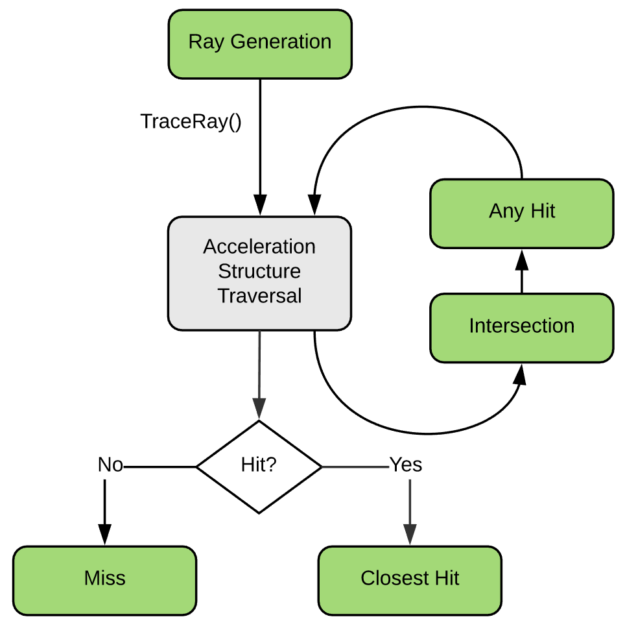
\includegraphics[scale=0.5]{RayTracing-Pipeline}
    \end{center}
    \caption{
        The Ray Tracing Pipeline.
        Green boxes are programmable functions and gray boxes are fixed functions in hardware.
        \parencite{NVIDIA:DXR-Intro}
    }
    \label{fig:RayTracing-Pipeline}
\end{figure}

The ray tracing pipeline is shown in Figure \ref{fig:RayTracing-Pipeline}.
Nearly all the stages in the pipeline are programmable, which allows the programmer to customize their ray tracing algorithm.
The hardware acceleration structure traversal is the most critical step because it requires the most computation.
It is fully implemented in hardware and is not programmable until it reaches the leaf nodes of the BVH, where the intersection stage is invoked.
Intersection stage reports if there is an intersection with the primitive in the bounding volume.
For triangles primitives, the intersection stage is implemented in hardware.
For AABB primitives, the stage is programmable, which this essay will utilize to intersect voxels.


This is because, AABBs are meant to enclose programmer defined primitives, such as spheres or abstract shapes while also utilizing hardware acceleration.
These programmer defined primitives are the leaf nodes of the BVH, thus hardware acceleration is leveraged until the leaf node is reached, where the programmer's intersection function is invoked
\parencite{NVIDIA:BVH-Patent}.
The acceleration structure traversal and intersection stage are repeated until the closest hit is found, because the first hit candidate could be occluded by another object.
Other stages in the pipeline are not as critical as the intersection stage and used to calculate the color of the pixel, which is not the focus of this essay.

\parencite{NVIDIA:RTGems2}

\section{Methodology}

Writing an application of this scope requires a deep understanding of the hardware, memory, graphics application programming interfaces (GAPI), graphics programming languages, debugging, etc.
This is because the GAPI are designed for industry professionals with years of experience working with GPUs.
Furthermore, debugging is non-trivial, because the algorithms are executed on the GPU, which cannot be debugged with traditional debugging tools.
Understanding all of these topics comfortably may require years of experience.

More than 3000+ lines of code are in the final implementation not accounting for rewrites of algorithms, debugging, and testing.

\subsection{Utilizing Hardware Acceleration}

This essay will use AABBs as voxels, because the GPU only accepts either triangles or AABBs as primitives.
Voxels are easily represented as AABBs, because both are cuboids.
The other alternative, representing voxels as triangles is not practical. Voxels have 6 faces, 2 triangles
are needed to represent each face, thus 12 triangles are needed to represent a voxel. This amounts to
inefficent memory usage and computation. Usage of AABBs implies that the programmer has to write the intersection function.

Acceleration structure generation is a black box in GAPIs, where
the primitives are supplied to the GPU and it constructs the AS. This is convenient to both the programmers and vendors, because
vendors can optimize the AS construction and traversal for their hardware and developers are ensured that the AS has optimal performance.

\subsection{Optimizing the Intersection Function}
\label{sec:OptimizingIntersection}

This section provides an optimization for the intersection stage,
which involves approximating the closest hit.

According to the specifications, the GPU may invoke an intersection functions for every AABB along the ray in no particular order \parencite{DirectX:Specification}.
This wastes computation for candidates that are not the closest hit.
The intersection function must be performant as it can be invoked many times for every ray.

\begin{figure}[H]
    \begin{center}
        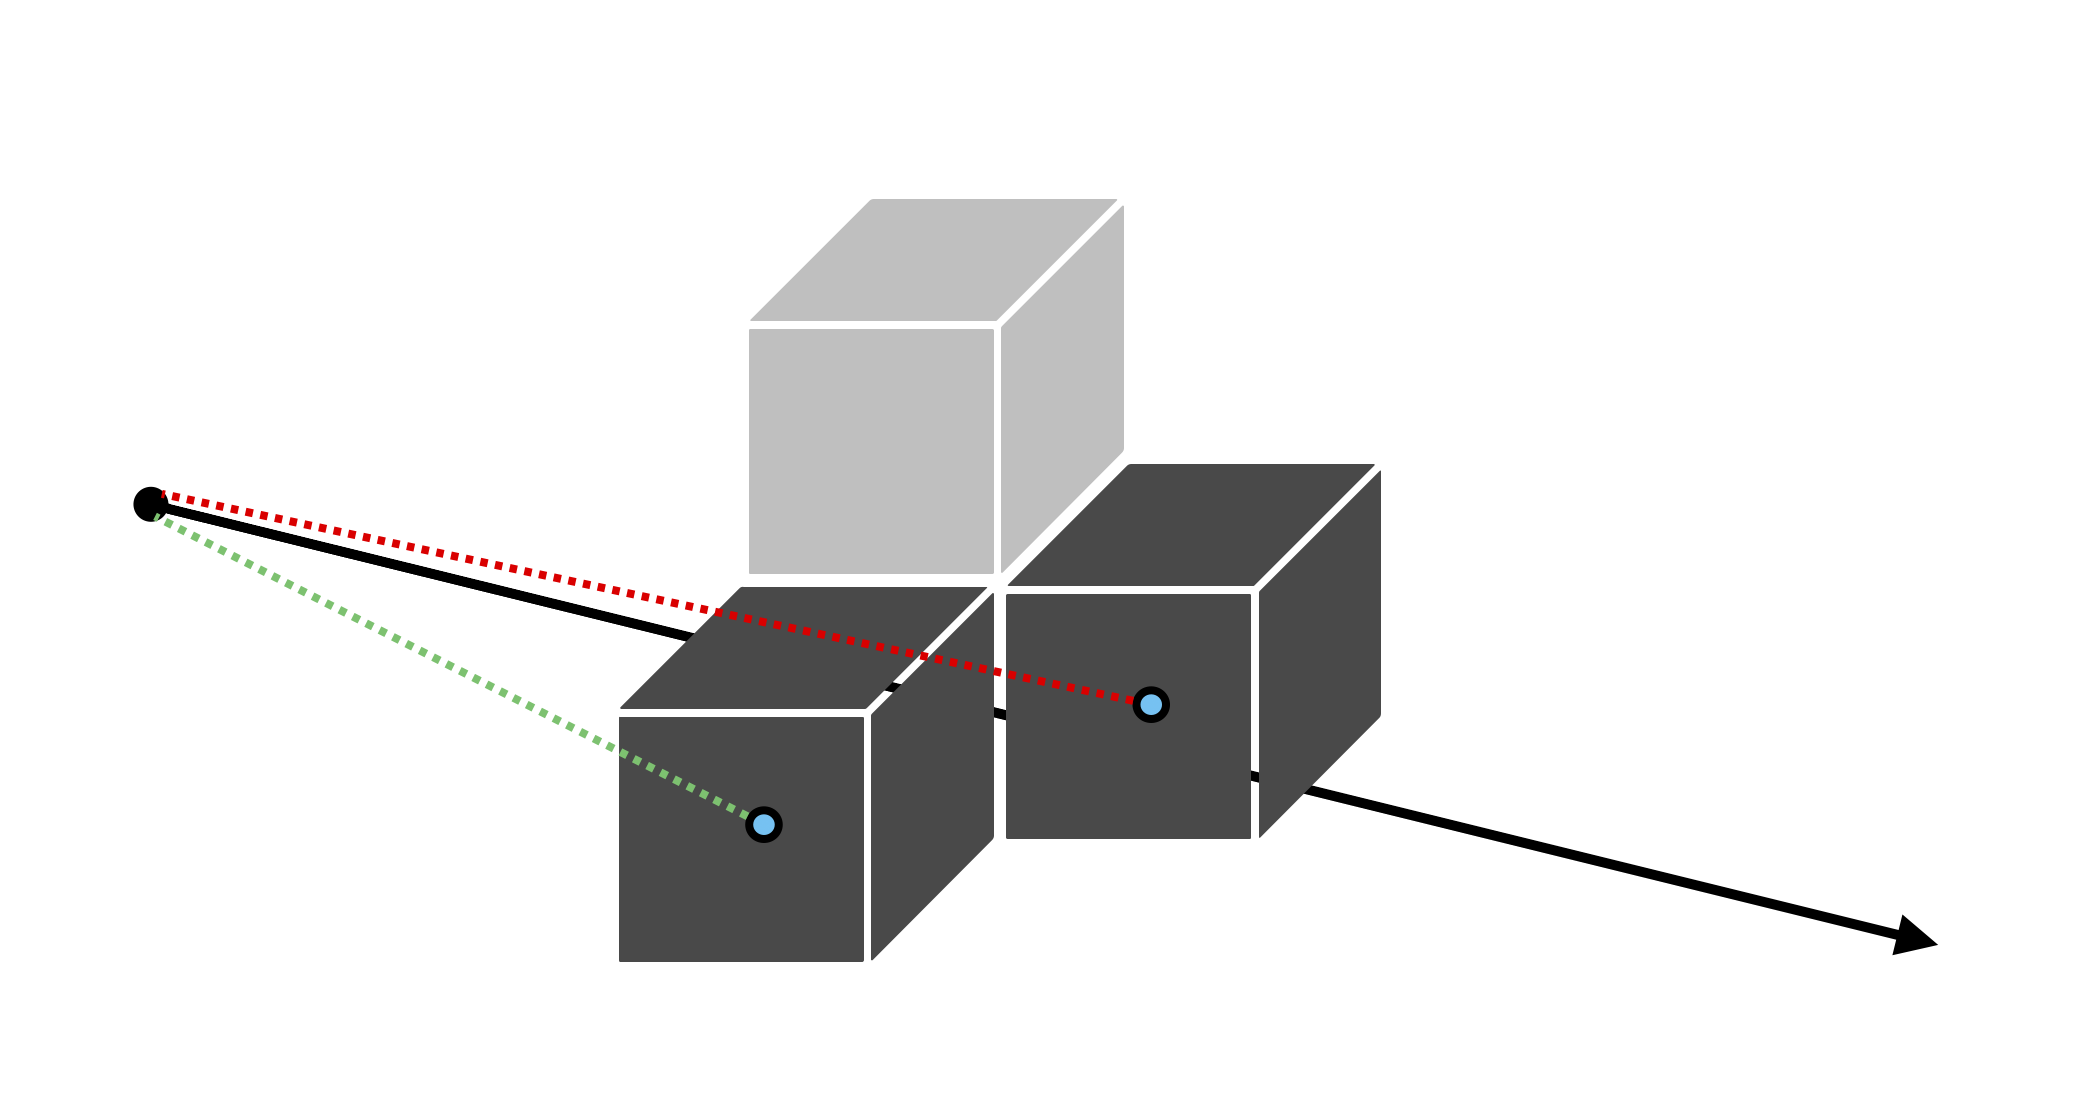
\includegraphics[scale=0.22]{ClosestHit-Approx}
    \end{center}
    \caption{
        Solving for closest hit candidate without a rigorous intersection test.
        Black voxels are the candidates hit along the ray.
        Dotted lines represent the distance from the ray origin to the voxel center.
    }
    \label{fig:ClosestHit-Approx}
\end{figure}

Figure \ref{fig:ClosestHit-Approx} shows solving for the closest candidate without a rigorous intersection test.
Solving the exact intersection for every candidate is not necessary, because the primitives are voxels.
Each voxel is a different distance from the ray origin, and the closest hit candidate is the voxel that is closest to the ray origin.

Because of this, the distance from the ray origin to the voxel center is calculated for every candidate, and the candidate with the smallest distance is selected.
After the closest candidate is found, the exact intersection can be calculated in the closest hit stage, because there is enough information to solve the exact intersection point.
Only one exact solution is calculated instead of many.
Fetching the voxel center is an array fetch and calculating the distance is a simple vector instruction, which is extremely fast.

\subsection{Memory Consumption}

The memory consumption is greater for AABBs than for voxels, because voxels can be represented by the center and the size.
This is 4 floats or 16 bytes per voxel. 3 floats for the x, y, and z coordinates of the center and 1 float for the size.
Unfortunately, the GPU requires AABBs to be used for hardware acceleration.
AABBs need two 3D vectors to represent the minimum and maximum points of the cuboid.
This is 6 floats or 24 bytes per AABB.
If there is a scene with 1 million voxels, then the memory consumption would be 24 MB.
This may not sound like much, however the AS has extra AABBs for the hierarchy, which will add up to more memory.
To do lighting calculations and other operations, the programmer would need to access the data specific to the voxel.
The GAPI does not allow accessing the data inside the AS. Thus, the programmer has to duplicate the data for the voxels in a separate
memory location, which will add up to roughly double the memory consumption.
This depletes the memory budget unnecessarily for applications on a tight memory budget.

\subsection{Data Collection}

Data collection to analyze the performance is done by measuring the frame time, frames per second (FPS), and memory consumption.
There are 3 different scenes with varying number of voxels to draw conclusions from.
These scenes are 3D scans of the real-world location that were in the form of polygons, because 3D model sharing
is universally done in the form of polygons. Real-world locations are chosen to represent practical applications utilizing
voxels for visualization. The scenes were converted to voxels by using FileToVox software \parencite{Github:FileToVox}.
The final code that is used in this essay can be found in the repository \citetitle{Github:FastVoxels} \parencite{Github:FastVoxels}.

\begin{itemize}
    \itemsep0em
    \item New York City: 4.3 million voxels \parencite{SketchFab:NewYorkCity}
    \item Operating Room: 5.2 million voxels \parencite{SketchFab:OperatingRoom}
    \item Church: 13.6 million voxels \parencite{SketchFab:Church}
\end{itemize}

The ray tracing algorithm is run for 4096 frames, and the average frame time is calculated.
Each ray can at most bounce 4 times, so the maximum recursion depth is 4.
Rays can terminate before reaching the maximum recursion depth if they hit a light source or the sky.
From the average frame time, the average frames per second (FPS) is calculated, by $FPS = \frac{1}{Average Frame Time}$,
which gives the number of frames that is rendered in a second.

Two methods of intersection tests are used:
\begin{itemize}
    \itemsep0em
    \item Exact Intersection: The exact intersection is calculated for every voxel.
    \item Approximate Intersection: The closest hit is approximated and the exact intersection is calculated in the closest hit stage.
          Described in Section \ref{sec:OptimizingIntersection}.
\end{itemize}

These methods are used to evaluate if the optimization yields any performance improvements compared to the exact intersection method.
Approximate method may improve the performance thus feasibility in real-time applications.

\section{Results}

This essay's analysis is based upon NVIDIA RTX 3060ti GPU on Windows 11 using DirectX 12.
Results may vary on different hardware and software configurations.
The GPU is one of the most common consumer GPUs according to {\it Steam Hardware Survey} \cite{Steam:HardwareSurvey}.

\subsection{Driver Conformance}

GAPIs such as Vulkan and DirectX 12 have strict specifications that the driver must conform to.
NVIDIA's GPU driver has been found not to conform strictly to either the Vulkan or DirectX 12 specification.

Wrong information about the AABB that was hit is passed to the intersection and closest hit stages.
The driver was merging voxels that were close to each other, into a single wide AABB.
It is important to note, that the driver may merge the AABBs for optimization, but it should still act as if the AABBs were not merged.
However, it behaved like a single wide AABB, which is illegal according to the specification \parencite{DirectX:Specification}.

\begin{figure}[H]
    \begin{center}
        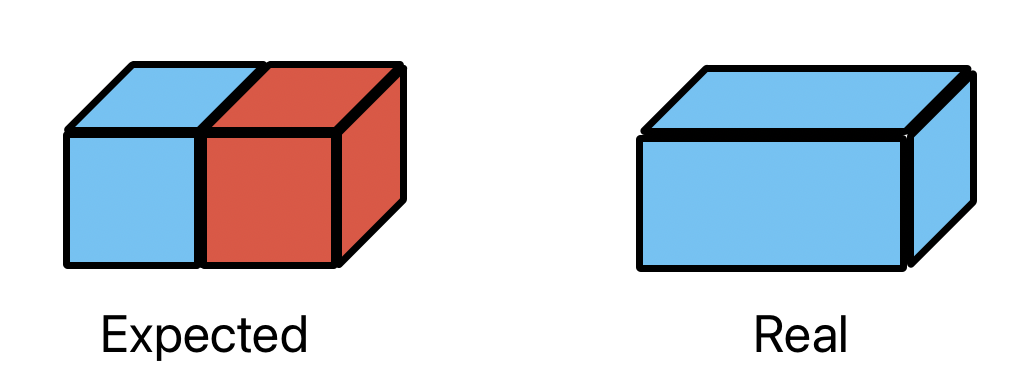
\includegraphics[scale=0.5]{Voxel-Merging}
    \end{center}
    \caption{
        The expected behavior compared to the real behavior.
    }
    \label{fig:Voxel-Merging}
\end{figure}

The merged AABB in Figure \ref{fig:Voxel-Merging} is blue,
because the driver reports that the primitive hit is the blue voxel even for the right side of the merged AABB.

The exact intersection method is not affected by this issue.
For the sake of this essay, the issue is ignored because the issue has been reported to NVIDIA, however,
the usability of the approximate method is severely impacted by this issue if not resolved.
This issue is not unique to this essay, as few developers have reported the same issue \parencite{NVIDIA:AABB-Merging}.
The code used in this essay has been written on Vulkan, and DirectX 12 GAPIs, and the issue was present in both.
Rewriting for a different GAPI was a monumental task, as the application required a complete rewrite of the C++ code.

\begin{figure}[H]
    \begin{center}
        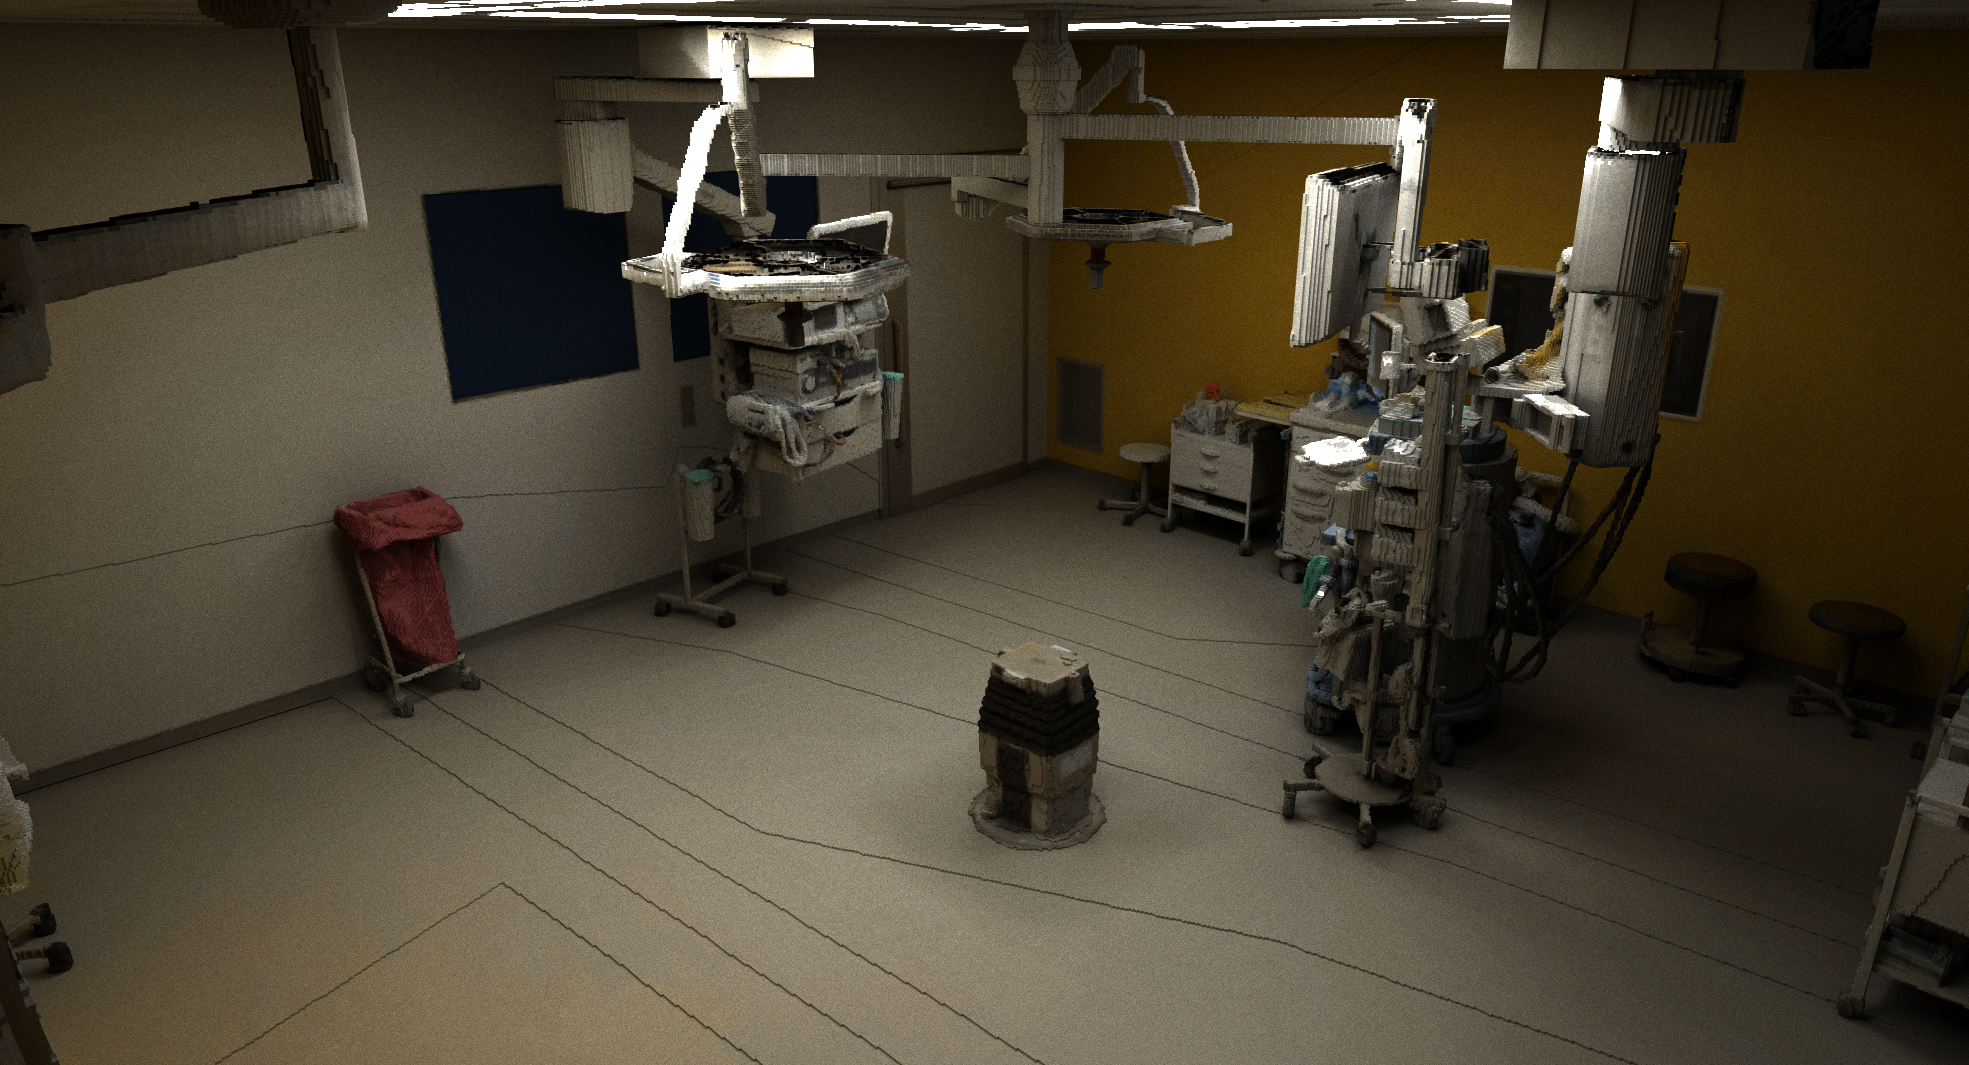
\includegraphics[scale=0.25]{OperationRoom.png}
        \smallbreak
        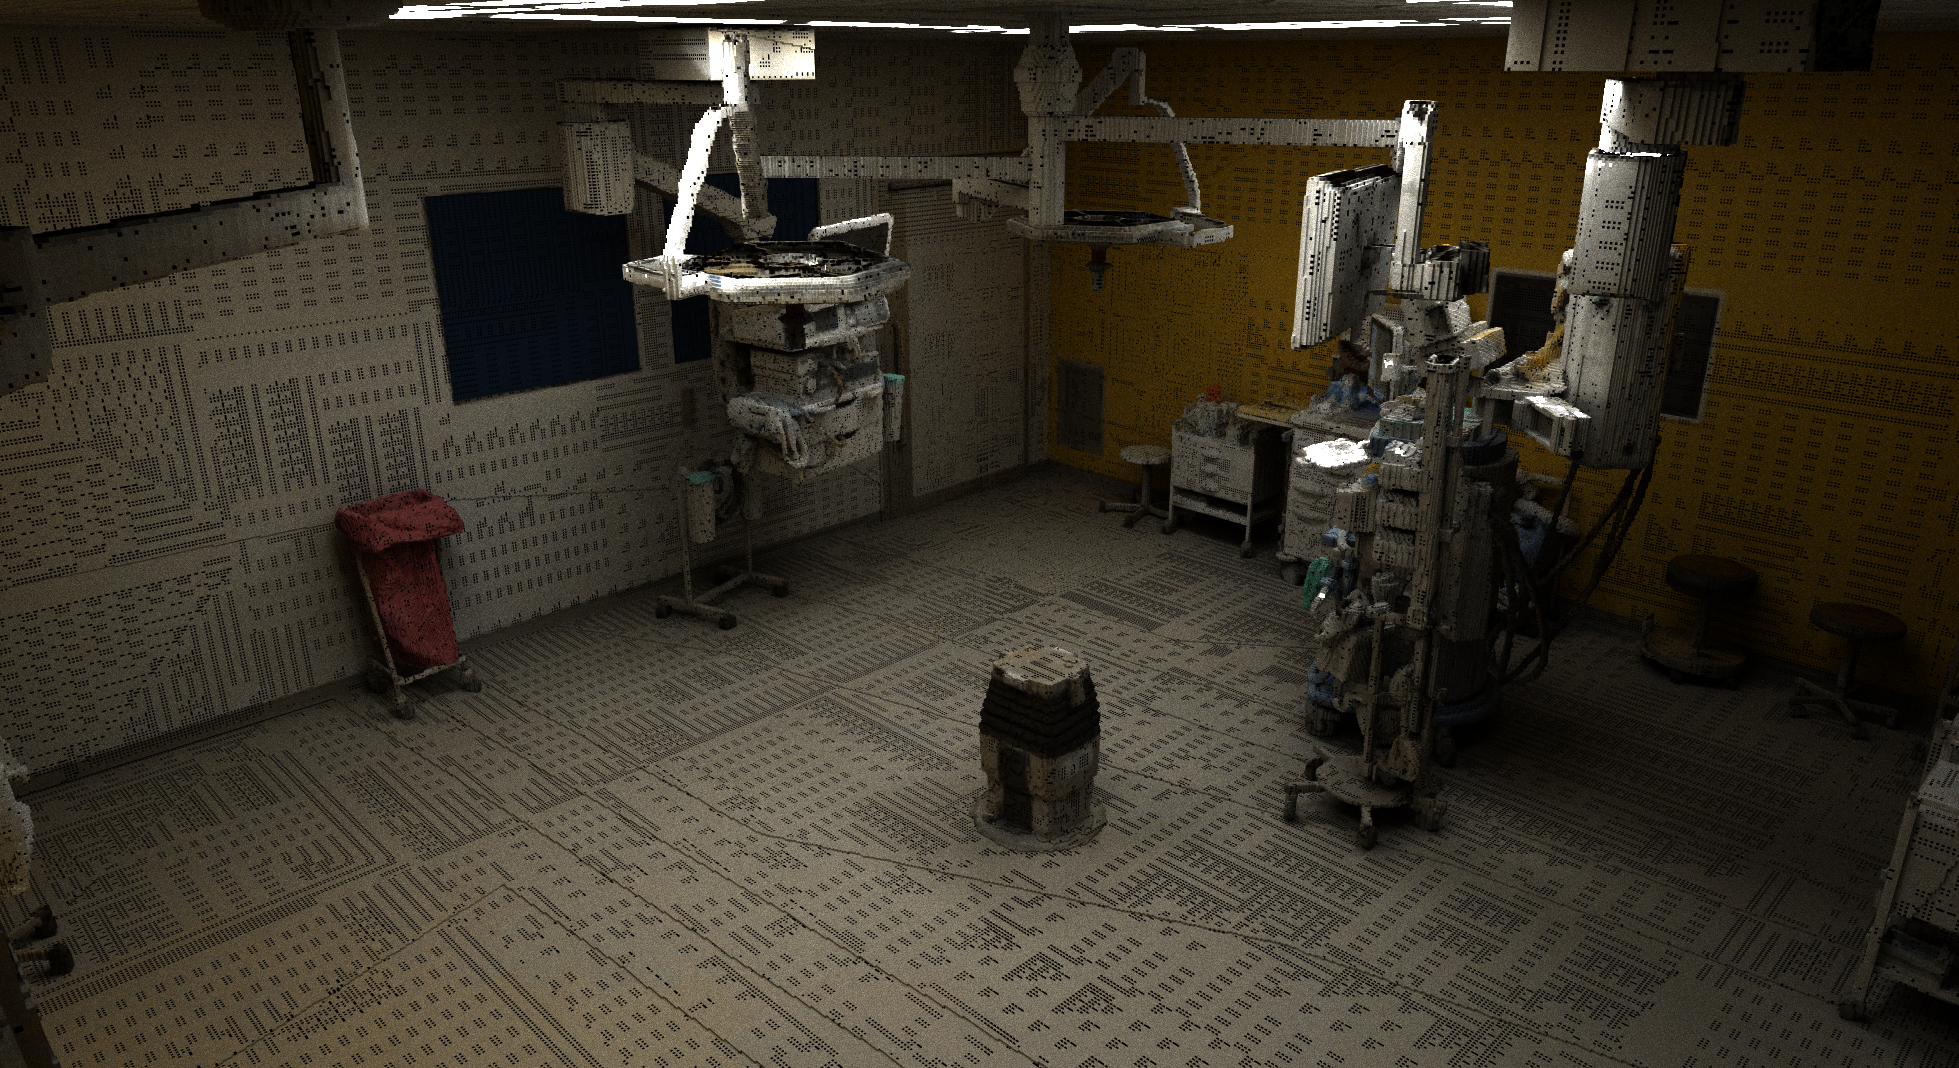
\includegraphics[scale=0.25]{OperationRoom-Merging}
    \end{center}
    \caption{
        Operating Room Scene - Exact Intersection (Top) and Approximate Intersection (Bottom).
        Black voxels are artifacts from the merging issue, present only in the approximate intersection method.
    }
    \label{fig:Scenes-Merging}
\end{figure}

\subsection{Stability}

While collecting data, the stability of the GPU was suboptimal. The GPU crashed multiple times
during data collection and after the data was collected.
The crashes were severe, as the system had to be restarted. Most of the crashes occurred
when collecting data for the Church and Operating Room scenes. It would end prematurely before the 4096 frames were rendered.
The CPU was going through 4096 frames, however, the GPU was not presenting the frames to the screen.
The data presented are from the runs that were not followed by a crash and did not cause any crashes.
This is relevant for the feasibility in real-time applications, because the system should not crash during rendering.

\subsection{Performance Data}

The data presented is relevant to evaluate the feasibility based on aforementioned criteria.

Formulas for calculating the changes are as follows:

Table \ref{tab:Performance-Milliseconds}:
$Change ~ (ms) = Approx - Exact$

Table \ref{tab:Performance-Frames}:
$Change ~ (\%) = \frac{Approx - Exact}{Exact} * 100$

Table \ref{tab:Memory-Consumption}:
$Change ~ (\%) = \frac{Accel. Struct. - Voxels}{Voxels} * 100$

\begin{table}[H]
    \centering
    \caption{Performance Data in Milliseconds. Lower is better.}
    \vspace{0.5cm}
    \label{tab:Performance-Milliseconds}
    \begin{tabular}{c||c|c|c|}
        Scene (voxels)           & Exact Int. & Approx Int. & Change (ms) \\ \toprule
        New York City (4.3 mil)  & 3.07       & 3.53        & +0.46       \\
        Operating Room (5.2 mil) & 10.7       & 10.0        & -0.7        \\
        Church (13.6 mil)        & 12.5       & 12.4        & -0.1        \\
    \end{tabular}
\end{table}

\begin{table}[H]
    \centering
    \caption{Performance Data in Frames Per Second. Higher is Better}
    \vspace{0.5cm}
    \label{tab:Performance-Frames}
    \begin{tabular}{c||c|c|c|}
        Scene (voxels)           & Exact Int. & Approx Int. & Change (\%) \\ \toprule
        New York City (4.3 mil)  & 324        & 282         & -13         \\
        Operating Room (5.2 mil) & 93         & 100         & +7.5        \\
        Church (13.6 mil)        & 80         & 81          & +1.3        \\
    \end{tabular}
\end{table}

% Approx NYC:                3.53 : 282
% Approx Operation Room:     10.0 : 100
% Approx Church:             12.4 : 81

% Exact NYC:            3.07 : 324
% Exact Operation Room: 10.7 : 93
% Exact Church:         12.5 : 80

% Memory NYC:                162725888 (AS) : 139198464 (Voxels)
% Memory Operating Room :     195952640 (AS) : 167706624 (Voxels)
% Memory Church:             513212416 (AS) : 438829056 (Voxels)

\begin{table}[H]
    \centering
    \caption{Memory Consumption in Megabytes. Lower is Better}
    \vspace{0.5cm}
    \label{tab:Memory-Consumption}
    \begin{tabular}{c||c|c|c|c|}
        Scene (voxels)           & Voxels & Accel. Struct. & Total & Change (\%) \\ \toprule
        New York City (4.3 mil)  & 139    & 162            & 301   & +16.5       \\
        Operating Room (5.2 mil) & 167    & 195            & 362   & +16.7       \\
        Church (13.6 mil)        & 438    & 513            & 951   & +17.1       \\
    \end{tabular}
\end{table}

\begin{figure}[H]
    \begin{center}
        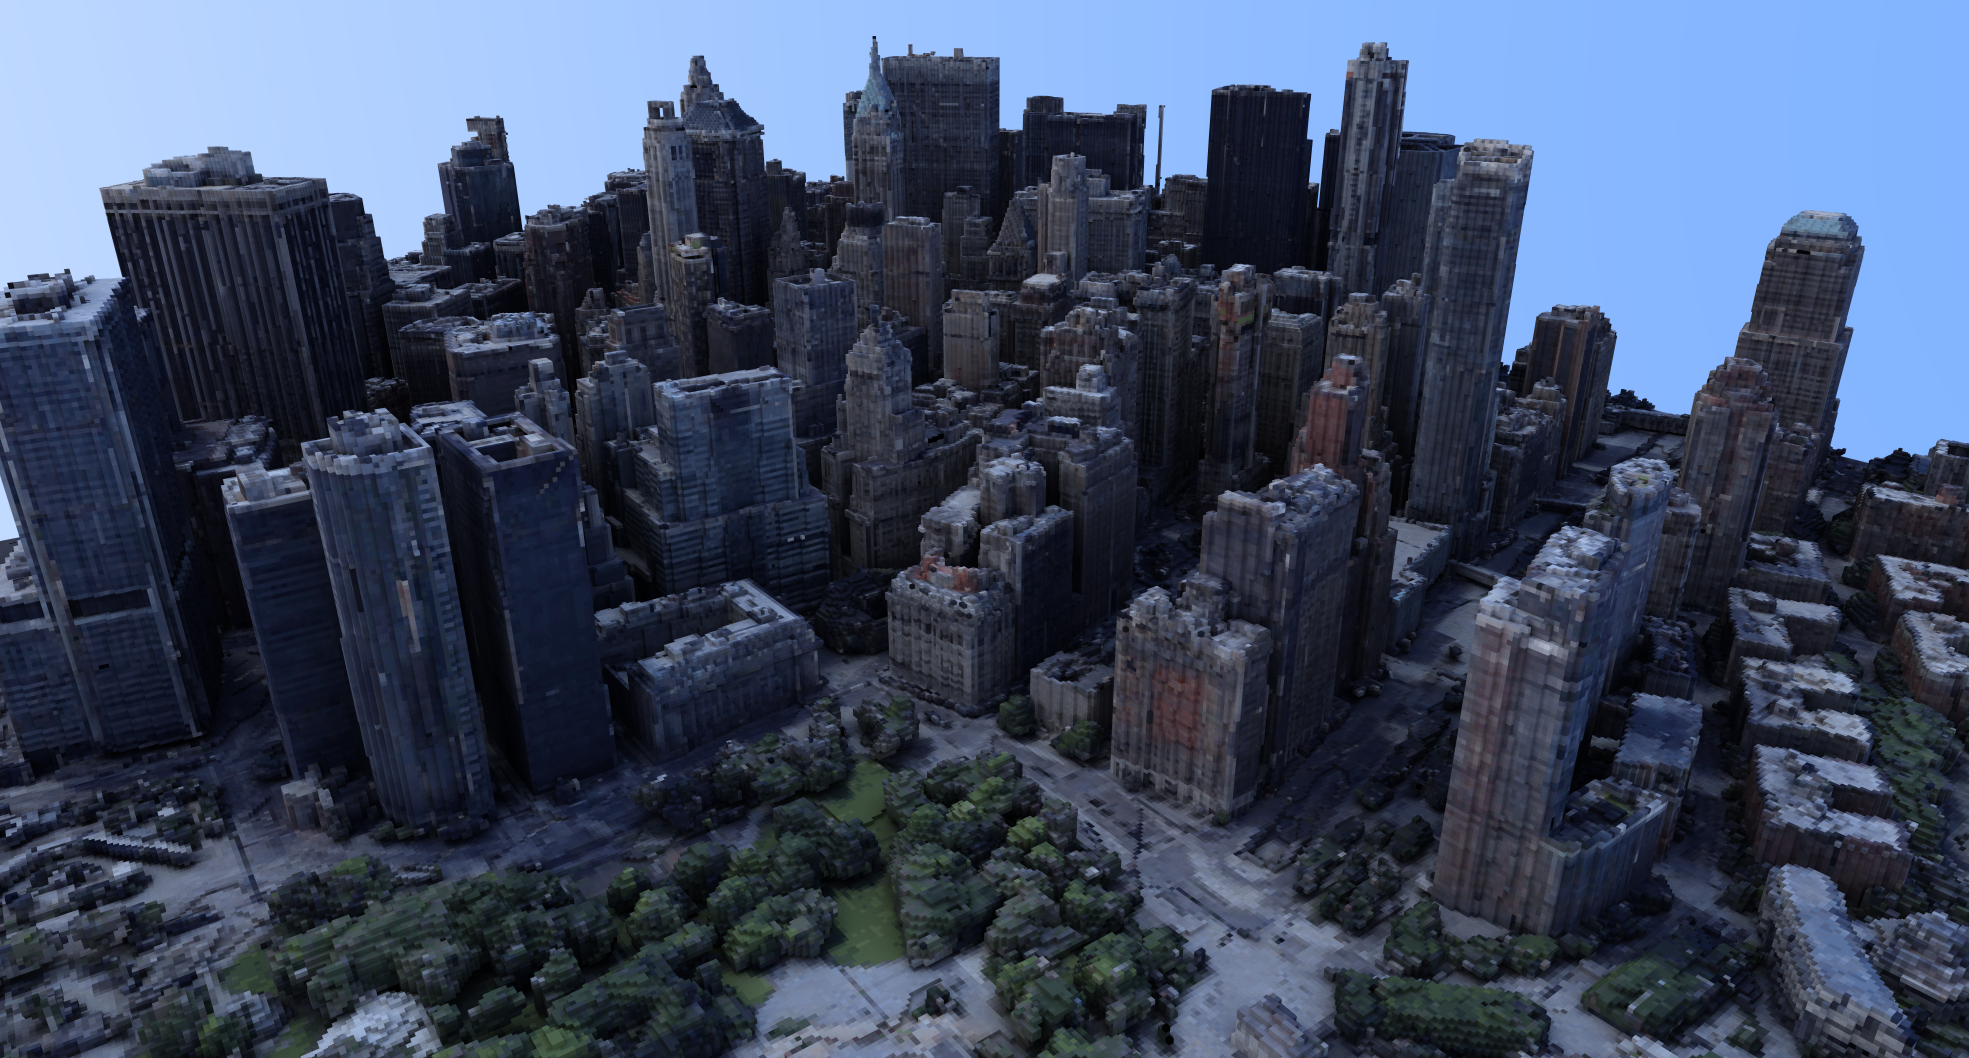
\includegraphics[scale=0.25]{NewYorkCity}
    \end{center}
    \caption{New York City Scene - Exact Intersection}
    \label{fig:NewYorkCity}
\end{figure}


\begin{figure}[H]
    \begin{center}
        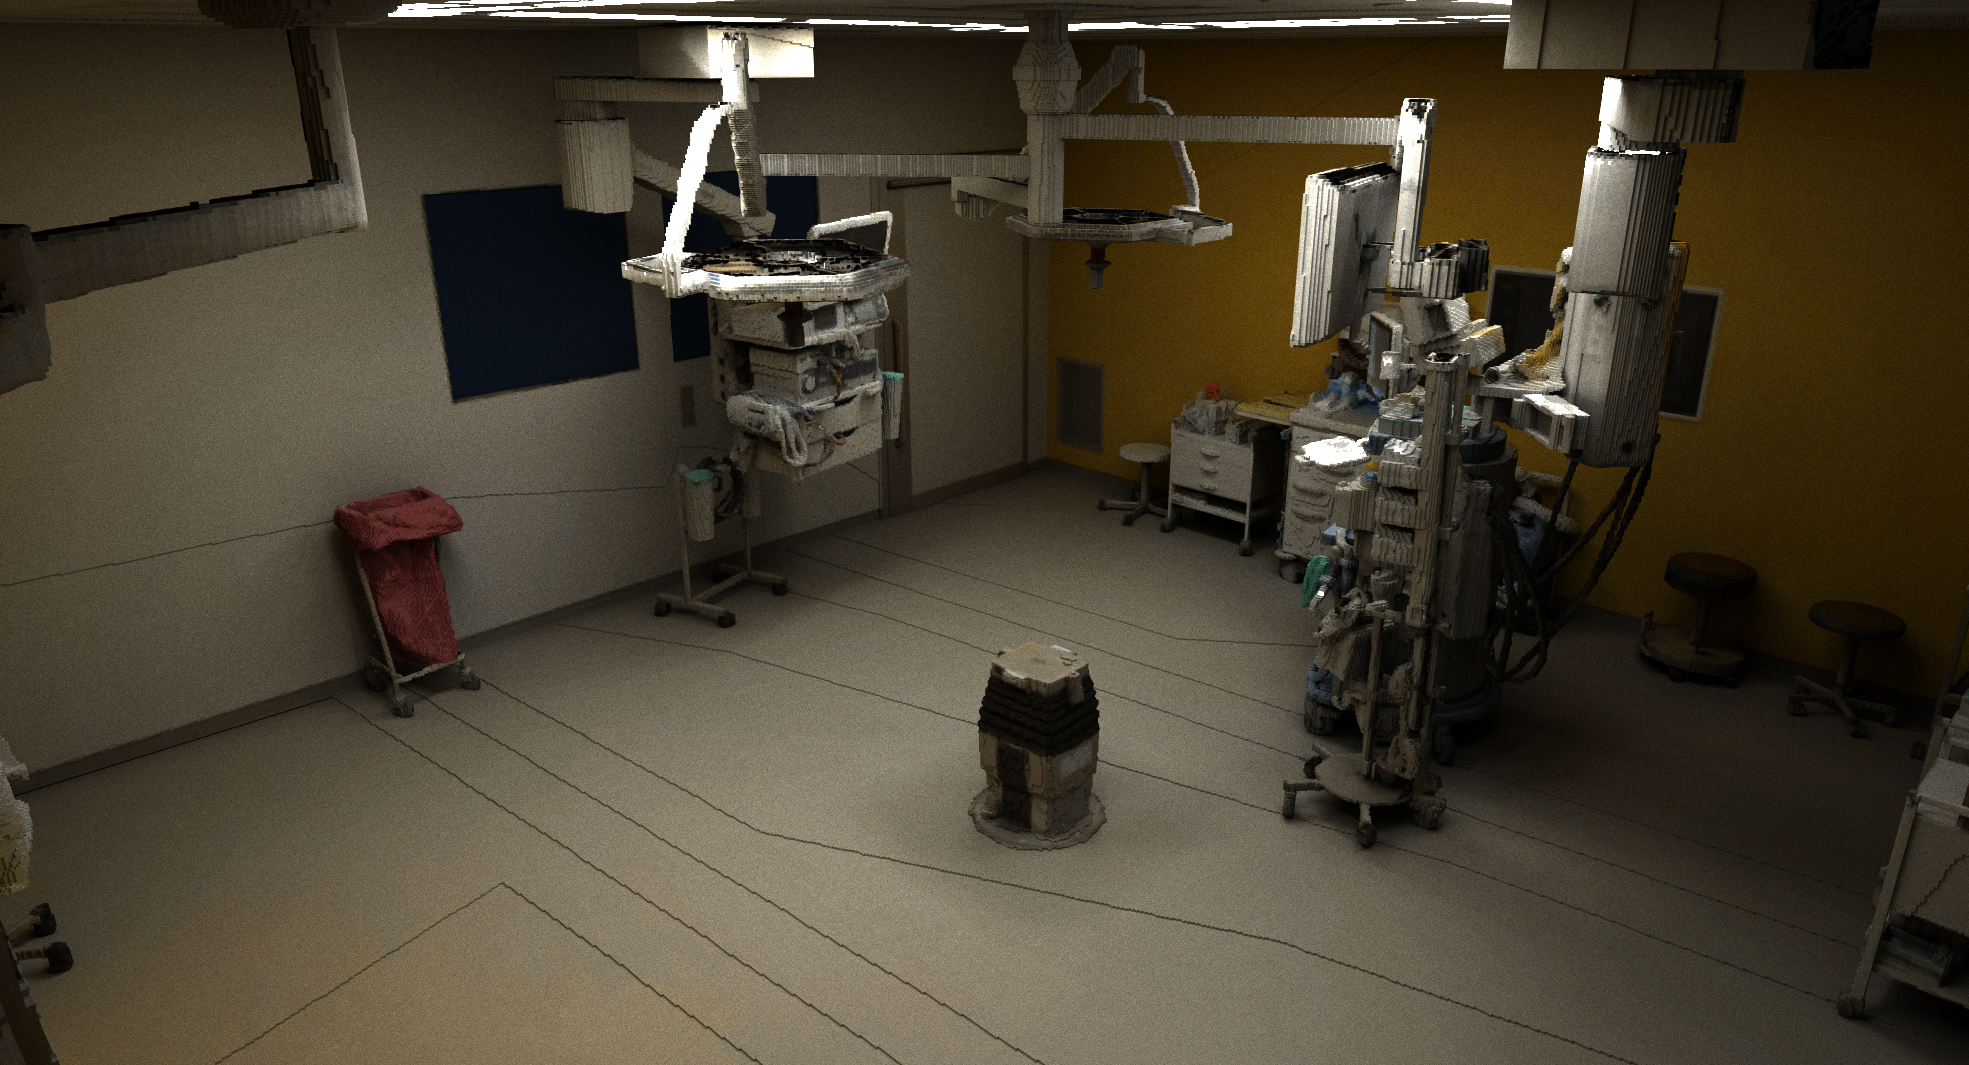
\includegraphics[scale=0.25]{OperationRoom}
    \end{center}
    \caption{Operating Room Scene - Exact Intersection}
    \label{fig:OperationRoom}
\end{figure}

\begin{figure}[H]
    \begin{center}
        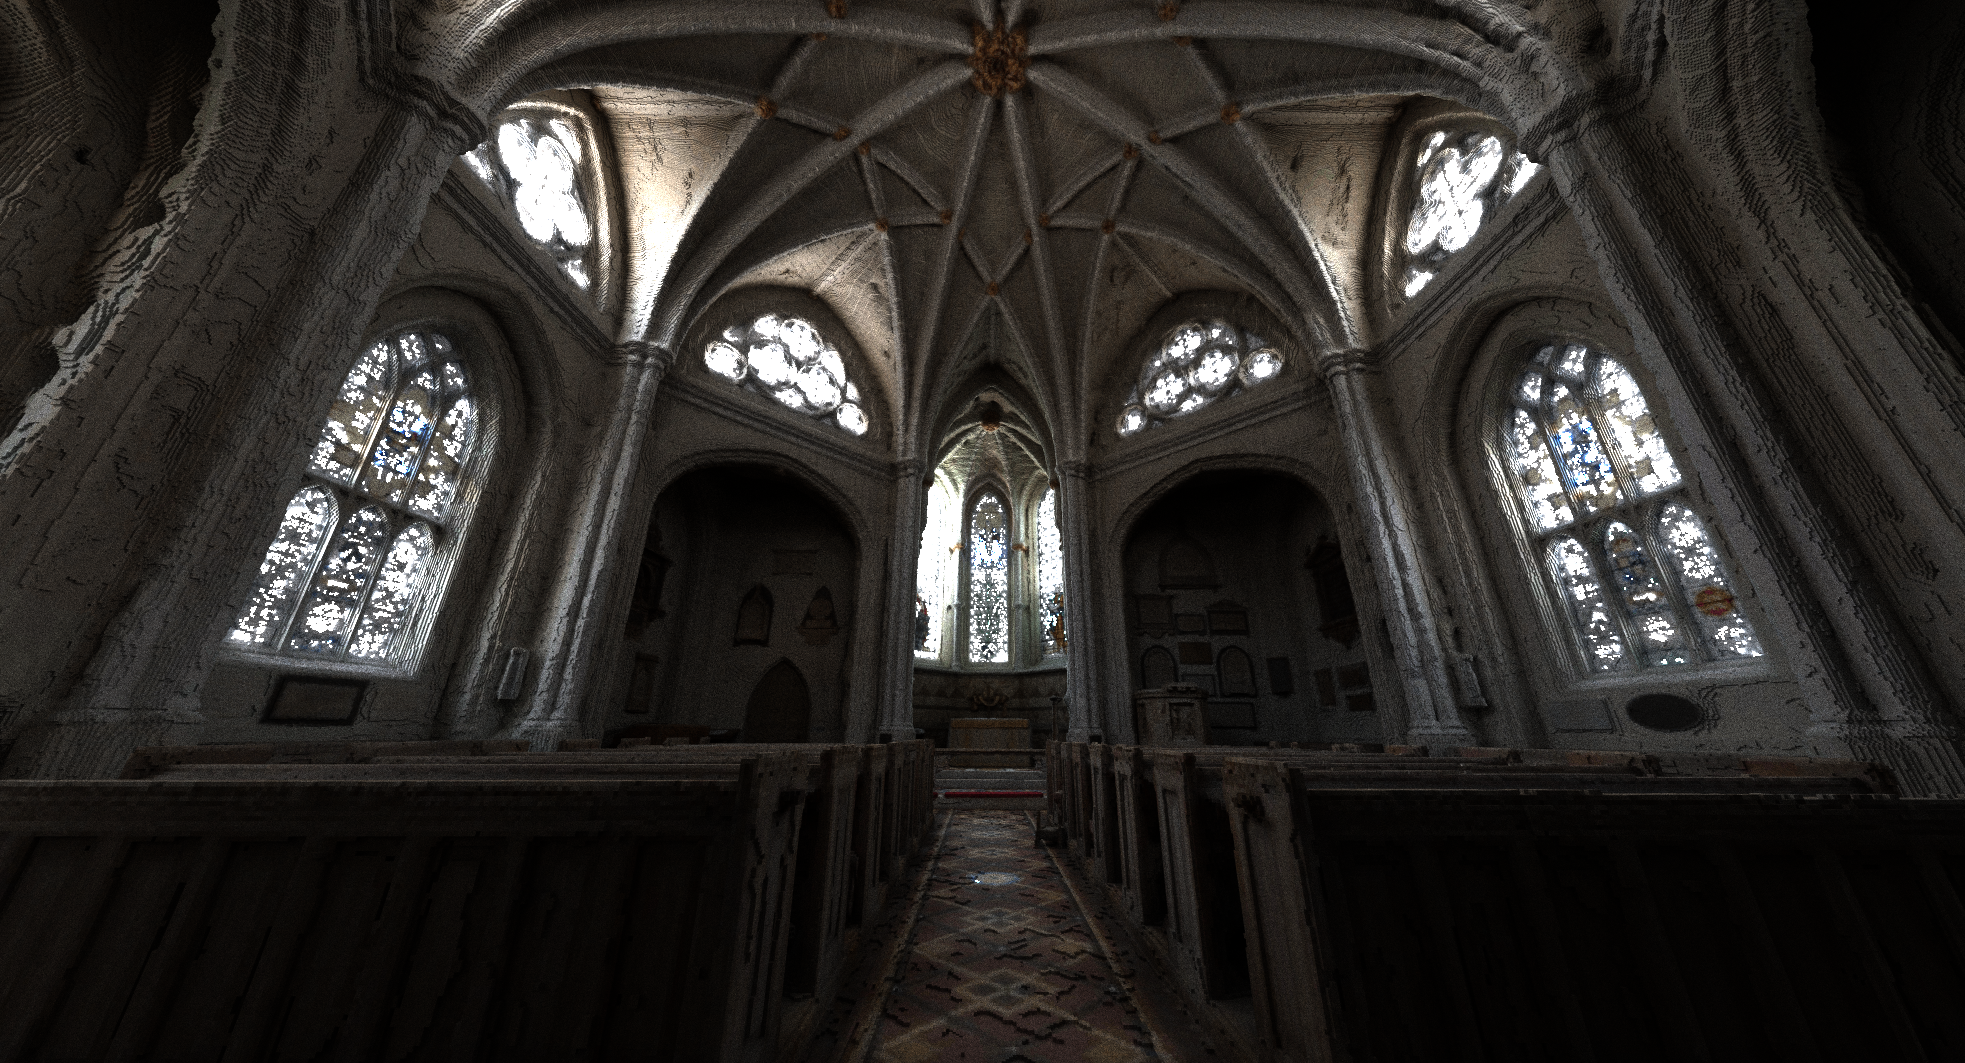
\includegraphics[scale=0.25]{Church}
    \end{center}
    \caption{Church Scene - Exact Intersection}
    \label{fig:Church}
\end{figure}


\subsection{Analysis of Results}

The results show that performance is excellent for all three scenes as they meet and exceed the target frame rate of 60 FPS.
Furthermore, the memory consumption is below 1 GB for all the scenes, which leaves memory for other tasks.

New York City scene has the lowest frame time of 3.07 ms for the exact intersection method.
The scene has the least number of voxels (4.3 million), and is open, meaning the rays can escape the scene quickly, resulting in less rays traced and less intersection tests.
Most of the rays bounce only once or twice before escaping the scene, resulting in low frame time.
The approximate intersection method is 0.46 ms slower, which is contrary to the expectation that the approximate intersection method would be faster.
This is a significant change, as FPS drops by 13\%, from 324 to 282.
In the source code, the approximate intersection method has fewer instructions to execute, however the exact intersection method is faster.
This would need further investigation to understand why the approximate intersection method is slower.
Despite the surprising results, it is favorable that the exact intersection method is more performant, because it does not suffer from artifacts caused by the driver issue.

Operating Room scene has only 1 million more voxels than the New York City scene, however the frame time for the exact intersection method is 10.7 ms, which is approximately 3 times slower in comparison.
This is caused by the enclosed environment where the rays can not escape the scene, thus have to either hit a light source, or bounce until the maximum recursion depth is reached before terminating.
Since the increase in frame time is not proportional to the increase in the number of voxels, it is evident that the closed environment increases the frame time significantly.
Contrary to the New York City scene, the approximate intersection method is faster in the Operating Room scene by 0.7 ms.
The optimized method does yield extra performance as the FPS increases by 7.5\%, from 93 to 100.
This is evidence that the optimization method works, but may not be advantageous in all scenes.

Church scene is the most complex scene with 13.6 million voxels. It is also enclosed like the operating room scene.
The frame time is 12.5 ms, which is approximately 2 ms slower than the operating room scene, even though the scene has twice the number of voxels than the operating room scene.
This proves that the frame time does not scale linearly with the number of voxels, thus acceleration structure traversal is extremely efficient.
In this case, the approximate intersection method is only 0.1 ms faster, which is not significant and may be within the margin of error.
Therefore, supporting the claim that the optimization may not perform better in all scenes.

The memory consumption is reasonable and below 1 GB for all the scenes.
However, it nearly crosses the 1 GB threshold for the Church scene with 951 MB.
If there did not need to be duplicated data, the memory consumption would not have gotten close to 1 GB.
An interesting observation is that the acceleration structure consumes 16-17\% more memory than the raw voxel data, regardless of the scene complexity.
This is caused by the extra AABBs for the hierarchy in the acceleration structure.
There is a linear relationship between the number of voxels and the memory consumption, which is expected.
It is more than the expectation of 24 MB for 1 million voxels, because the voxels contain auxiliary data such as color.

\section{Conclusion}

Results show that hardware accelerated voxel ray is feasible on consumer hardware for real-time applications.
It both handles a reasonable number of voxels that would be used in real-time applications and does not exceed the memory budget of 1 GB.
The exceptional performance also leaves room for other tasks such as AI, physics calculations and post-processing which are common in real-time applications.
Increase in the scene complexity does not scale linearly with the frame time, which allows for even more complex scenes
to be ray traced than the ones used in this essay, with looser constraints on the frame time and memory budget.
However, unless the stability improves, it is not practical to build applications with high complexity scenes,
because it is prone to severe crashes.

The optimization method in this essay does improve frame time, but not in all scenes, closed environments show improvement, while open environments do not.
However, the difference is not significant, which may be caused by the driver optimizing and only invoking the intersection function for the closest few candidates.
The approximate method is only preferable if the driver issue is resolved.
Furthermore, the memory consumption is reasonable and within the budget, but can be further reduced,
if GAPIs allowed access to the AABB data inside the acceleration structure, which would eliminate the need for duplicate data.

Ultimately, the results show that hardware accelerated voxel ray is feasible on consumer hardware for real-time applications,
and extremely performant, even for complex scenes, but stability issues need to be resolved for practical applications.

\printbibliography

\end{document}